\documentclass[]{article}

\usepackage{amsmath}
\usepackage{amsfonts}
\usepackage{amsthm}
\usepackage{amssymb}
\usepackage{mathrsfs}
\usepackage{stmaryrd}
\usepackage{tikz}

\newcommand{\Q}{\mathbb{Q}}
\newcommand{\N}{\mathbb{N}}
\newcommand{\Z}{\mathbb{Z}}
\newcommand{\R}{\mathbb{R}}
\newcommand{\Primes}{\mathbb{P}}
\newcommand{\st}{\text{ s.t. }}
\newcommand{\txtand}{\text{ and }}
\newcommand{\txtor}{\text{ or }}
\newcommand{\lxor}{\veebar}
\newcommand{\vecx}{ \vec{\mathbf{x}} }
\newcommand{\vecxk}{ \vec{\mathbf{x_k}} }
\newcommand{\vecw}{ \vec{\mathbf{w}} }

%opening
\title{Notes on Binary Classification\\ \large Support Vector Machines and Logistic Regression}
\author{DSBA Mathematics Refresher 2026}
\date{}

\begin{document}

	\maketitle

	\begin{abstract}

	\end{abstract}

	This session is about \textbf{binary classification}: given a set of labelled examples, we want to build a rule that predicts the label of a new, unseen example.
	We will see two classical methods, which are also two applications of what we have done in the previous sessions:
	\begin{itemize}
		\item \textbf{Support Vector Machines}, which lead to a \textit{constrained} optimization problem (Constrained Optimization session);
		\item \textbf{Logistic regression}, which leads to an \textit{unconstrained} optimization problem, solved by gradient descent (Session 3).
	\end{itemize}

	\section{The Binary Classification Problem}

	Our data is a set of $N$ labelled points
	$$
	\left\{ \left(\vecxk, y_k\right) \right\}_{k=1}^{N}
	$$
	where $\vecxk \in \R^n$ describes the $k$-th example (its "features") and $y_k$ is its \textbf{label}.
	As there are only two classes, the label takes only two values, and it is convenient to write them
	$$
	y_k \in \{-1, +1\}
	$$

	\noindent \textbf{Example:}
	$\vecxk$ could be $\begin{pmatrix} \text{income} \\ \text{age} \end{pmatrix}$ of a customer, and $y_k$ whether that customer subscribed ($+1$) or not ($-1$).
	Given a new customer, we want to predict whether they will subscribe.

	We look for a rule of the form: compute some function $h(\vecx)$, and predict $+1$ if $h(\vecx) > 0$, and $-1$ if $h(\vecx) < 0$.
	The set $\{h(\vecx) = 0\}$ is the \textbf{decision boundary}.

	\section{Separating Hyperplanes}

	The simplest choice is a \textbf{linear} function:
	$$
	h(\vecx) = \vecw \cdot \vecx - b
	$$
	where $\vecw \in \R^n$ and $b \in \R$ are the parameters to be learned.
	In $\R^2$, $\{h(\vecx) = 0\}$ is a line; in $\R^3$ it is a plane; in general it is called a \textbf{hyperplane}.
	It cuts the space into two regions:
	$$
	\mathcal{R}_{-1} = \left\{ \vecx : \vecw \cdot \vecx - b < 0 \right\}
	\qquad \text{and} \qquad
	\mathcal{R}_{+1} = \left\{ \vecx : \vecw \cdot \vecx - b > 0 \right\}
	$$

	\paragraph{Handling the two labels at once}
	\noindent\\
	Classifying the point $\vecxk$ correctly means
	$$
	h(\vecxk) > 0 \ \text{ if } y_k = +1
	\qquad \text{and} \qquad
	h(\vecxk) < 0 \ \text{ if } y_k = -1
	$$
	In both cases $h(\vecxk)$ has the \textit{same sign} as $y_k$, so their product is positive, and the two conditions collapse into a single one:
	$$
	y_k \, h(\vecxk) > 0
	$$
	This trick (multiplying by the label $\pm 1$ to replace a case distinction by one inequality) is used constantly, and it is the reason for labelling the classes $-1$ and $+1$ rather than $0$ and $1$.

	\paragraph{Distance to the hyperplane}
	\noindent\\
	The vector $\vecw$ is perpendicular to the hyperplane.
	Therefore, if $\vecx_1$ is any point of the hyperplane (so that $\vecw \cdot \vecx_1 = b$), the distance from a point $\vecx_0$ to the hyperplane is the length of the projection of $\vecx_0 - \vecx_1$ onto the unit normal $\frac{\vecw}{\|\vecw\|}$:
	$$
	d(\vecx_0) = \left| \left(\vecx_0 - \vecx_1\right) \cdot \frac{\vecw}{\|\vecw\|} \right|
	= \frac{\left| \vecw \cdot \vecx_0 - b \right|}{\|\vecw\|}
	$$
	Note that this does not depend on which point $\vecx_1$ was chosen.

	\noindent \textbf{Example:}
	In $\R^2$ with $\vecw = \begin{pmatrix} 1 \\ 1 \end{pmatrix}$ and $b = \frac{3}{2}$, the hyperplane is the line $x + y = \frac{3}{2}$, and the distance from the point $(1,1)$ to it is
	$$
	\frac{\left| 1 + 1 - \frac{3}{2} \right|}{\sqrt{1^2+1^2}} = \frac{1/2}{\sqrt{2}} = \frac{\sqrt{2}}{4} \approx 0.354
	$$

	\section{Support Vector Machines}

	When the data is \textbf{linearly separable}, there are usually \textit{infinitely many} hyperplanes separating the two classes.
	Which one should we choose?

	The idea of the Support Vector Machine is to pick the one that leaves as much room as possible on both sides: the one \textbf{maximizing the margin}.

	\paragraph{The margin}
	\noindent\\
	Notice that $h$ and $2h$ define the same decision boundary: multiplying $\vecw$ and $b$ by the same positive number changes nothing.
	We can therefore fix the scale by requiring that the closest points satisfy $|h(\vecxk)| = 1$.
	The picture is then made of three regions:
	$$
	\mathcal{R}_{-1}: \ \vecw \cdot \vecx - b < -1,
	\qquad
	\mathcal{R}_{0}: \ \left| \vecw \cdot \vecx - b \right| < 1,
	\qquad
	\mathcal{R}_{+1}: \ \vecw \cdot \vecx - b > 1
	$$
	where $\mathcal{R}_0$ is the \textbf{margin band}, which should contain no data point at all.

	Its width is computed as follows: let $\vecx_-$ and $\vecx_+$ be two points, one on each edge, with $\vecx_+ - \vecx_- = d \cdot \frac{\vecw}{\|\vecw\|}$ perpendicular to both edges.
	Subtracting the two equations $\vecw \cdot \vecx_+ - b = 1$ and $\vecw \cdot \vecx_- - b = -1$:
	$$
	\vecw \cdot \left( \vecx_+ - \vecx_- \right) = 2
	\qquad \Longrightarrow \qquad
	d \, \|\vecw\| = 2
	\qquad \Longrightarrow \qquad
	d = \frac{2}{\|\vecw\|}
	$$

	\paragraph{The optimization problem}
	\noindent\\
	Requiring every point to be correctly classified \textit{and} outside the margin band is written, with the same trick as before,
	$$
	y_k \left( \vecw \cdot \vecxk - b \right) \geq 1
	\qquad \text{for all } k
	$$
	and maximizing the margin $\frac{2}{\|\vecw\|}$ means minimizing $\|\vecw\|$.
	The SVM is therefore the solution of
	$$
	\text{minimize } \ \frac{1}{2}\|\vecw\|^2
	\qquad \text{subject to} \qquad
	y_k \left( \vecw \cdot \vecxk - b \right) \geq 1 \quad \text{for all } k
	$$
	We minimize $\frac{1}{2}\|\vecw\|^2$ rather than $\|\vecw\|$ because it has the same minimizer and is much nicer to differentiate.

	This is exactly a constrained optimization problem with inequality constraints, of the kind studied in the Constrained Optimization session: it is solved with Lagrange multipliers (one per data point) and slack variables.
	The details are outside the scope of this course (in practice, we let a computer solve it).

	\paragraph{Support vectors}
	\noindent\\
	At the optimum, most constraints are \textit{inactive} (their multiplier is $0$): the corresponding points are strictly outside the margin band and play no role.
	The points for which $y_k h(\vecxk) = 1$ (those lying exactly on the edges of the band) are the \textbf{support vectors}, and they alone determine the solution.
	Moving or deleting any other point does not change the answer.
	This is where the method gets its name, and it is also what makes it economical: the model is described by a handful of points.

	\paragraph{A worked example}
	\noindent\\
	Take four points in $\R^2$:
	$$
	\text{class } +1: \ \vecx_1 = \begin{pmatrix} 3 \\ 1 \end{pmatrix}, \ \vecx_2 = \begin{pmatrix} 3 \\ -1 \end{pmatrix}
	\qquad
	\text{class } -1: \ \vecx_3 = \begin{pmatrix} 1 \\ 0 \end{pmatrix}, \ \vecx_4 = \begin{pmatrix} 0 \\ 2 \end{pmatrix}
	$$

	\begin{center}
		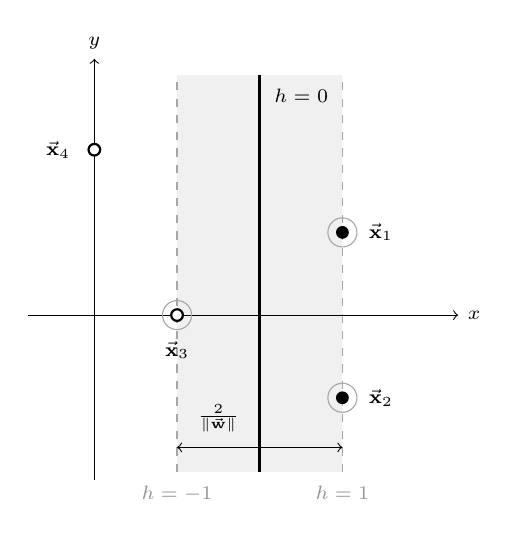
\begin{tikzpicture}[scale=1.05]
			% the margin band
			\fill[gray!12] (1,-1.9) rectangle (3,2.9);
			\draw[dashed,gray!70] (1,-1.9) -- (1,2.9);
			\draw[dashed,gray!70] (3,-1.9) -- (3,2.9);
			\draw[very thick] (2,-1.9) -- (2,2.9);
			\node[right] at (2.06,2.65) {\scriptsize $h=0$};
			\node[gray!85,below] at (1,-1.95) {\scriptsize $h=-1$};
			\node[gray!85,below] at (3,-1.95) {\scriptsize $h=1$};
			% axes
			\draw[->] (-0.8,0) -- (4.4,0) node[right] {\scriptsize $x$};
			\draw[->] (0,-2.0) -- (0,3.1) node[above] {\scriptsize $y$};
			% class +1
			\draw[gray!70] (3,1) circle (5pt);
			\draw[gray!70] (3,-1) circle (5pt);
			\filldraw (3,1) circle (2pt) node[right,xshift=6pt] {\scriptsize $\vecx_1$};
			\filldraw (3,-1) circle (2pt) node[right,xshift=6pt] {\scriptsize $\vecx_2$};
			% class -1
			\draw[gray!70] (1,0) circle (5pt);
			\filldraw[fill=white,thick] (1,0) circle (2pt) node[below,yshift=-6pt] {\scriptsize $\vecx_3$};
			\filldraw[fill=white,thick] (0,2) circle (2pt) node[left,xshift=-5pt] {\scriptsize $\vecx_4$};
			% the margin
			\draw[<->] (1,-1.6) -- (3,-1.6);
			\node at (1.5,-1.25) {\scriptsize $\frac{2}{\|\vecw\|}$};
		\end{tikzpicture}
		\\[0.3em]
		{\scriptsize Filled dots are the class $+1$ and open dots the class $-1$.
		The band drawn is the one computed below, and the circled points are its support vectors.}
	\end{center}

	\noindent \textbf{Step 1: write the problem.}
	Write $\vecw = \begin{pmatrix} w_1 \\ w_2 \end{pmatrix}$.
	The four constraints $y_k \left( \vecw \cdot \vecxk - b \right) \geq 1$ then read:
	$$
	g_1 = 3 w_1 + w_2 - b - 1 \geq 0,
	\qquad
	g_2 = 3 w_1 - w_2 - b - 1 \geq 0
	$$
	$$
	g_3 = b - w_1 - 1 \geq 0,
	\qquad
	g_4 = b - 2 w_2 - 1 \geq 0
	$$
	(the last two carry a minus sign because $y_3 = y_4 = -1$), and we minimize $\frac{1}{2} \|\vecw\|^2$.

	\noindent \textbf{Step 2: write the Lagrangian.}
	One multiplier and one slack variable per constraint, exactly as in the Constrained Optimization session.
	Written out in full:
	$$
	\begin{aligned}
		\mathcal{L}\left(w_1, w_2, b, s_1, \dots, s_4, \alpha_1, \dots, \alpha_4\right)
		= \ & \frac{1}{2} \left( w_1^2 + w_2^2 \right) \\
		& - \alpha_1 \left( 3 w_1 + w_2 - b - 1 - s_1^2 \right) \\
		& - \alpha_2 \left( 3 w_1 - w_2 - b - 1 - s_2^2 \right) \\
		& - \alpha_3 \left( b - w_1 - 1 - s_3^2 \right) \\
		& - \alpha_4 \left( b - 2 w_2 - 1 - s_4^2 \right)
	\end{aligned}
	$$
	Its partial derivatives, set to zero, are:
	$$
	\frac{\partial \mathcal{L}}{\partial w_1} = w_1 - 3\alpha_1 - 3\alpha_2 + \alpha_3 = 0,
	\qquad
	\frac{\partial \mathcal{L}}{\partial w_2} = w_2 - \alpha_1 + \alpha_2 + 2\alpha_4 = 0
	$$
	$$
	\frac{\partial \mathcal{L}}{\partial b} = \alpha_1 + \alpha_2 - \alpha_3 - \alpha_4 = 0,
	\qquad
	\frac{\partial \mathcal{L}}{\partial s_k} = 2 \alpha_k s_k = 0
	\quad \text{for } k = 1, \dots, 4
	$$
	and the four derivatives with respect to the $\alpha_k$ hand the constraints back, $g_k = s_k^2 \geq 0$.

	The first two say that $\vecw$ is built from the data:
	$$
	\vecw = \begin{pmatrix} 3\alpha_1 + 3\alpha_2 - \alpha_3 \\ \alpha_1 - \alpha_2 - 2\alpha_4 \end{pmatrix}
	= \alpha_1 \begin{pmatrix} 3 \\ 1 \end{pmatrix}
	+ \alpha_2 \begin{pmatrix} 3 \\ -1 \end{pmatrix}
	- \alpha_3 \begin{pmatrix} 1 \\ 0 \end{pmatrix}
	- \alpha_4 \begin{pmatrix} 0 \\ 2 \end{pmatrix}
	= \sum_{k=1}^{4} \alpha_k y_k \vecxk
	$$
	the third is the balance $\sum_k \alpha_k y_k = 0$ between the two classes, and each of the four $\partial \mathcal{L} / \partial s_k = 0$ says that $\alpha_k = 0$ \textit{or} $s_k = 0$, that is, the constraint $g_k$ is active.
	Adding the sign conditions $\alpha_k \geq 0$, these are the KKT conditions of the problem.
	Since the objective is convex and the constraints are linear, they are not only necessary but also \textit{sufficient}: as soon as we produce numbers satisfying all of them, we have the solution and we may stop searching.

	\noindent \textbf{Step 3: go through the cases.}
	Complementary slackness says that each $\alpha_k$ is zero \textit{or} its constraint is active, and we do not know in advance which points are which, so we try the possibilities in turn.

	\begin{enumerate}
		\item \textit{No constraint active}, so every $\alpha_k = 0$ and $\vecw = \vec{\mathbf{0}}$.
		Then $g_1 \geq 0$ and $g_3 \geq 0$ read $-b \geq 1$ and $b \geq 1$, which is impossible.
		Some multiplier is therefore positive, and by $\alpha_1 + \alpha_2 = \alpha_3 + \alpha_4$ each class carries at least one.

		\item \textit{One point of each class active}, say $\alpha_1, \alpha_3 > 0$ and $\alpha_2 = \alpha_4 = 0$.
		The second stationarity equation gives $\alpha_1 = \alpha_3 = \alpha$, hence:
		$$
		\vecw = \alpha \begin{pmatrix} 3 \\ 1 \end{pmatrix} - \alpha \begin{pmatrix} 1 \\ 0 \end{pmatrix} = \begin{pmatrix} 2\alpha \\ \alpha \end{pmatrix}
		$$
		Activity of $g_1$ and $g_3$ gives $b = 7\alpha - 1$ and $b = 2\alpha + 1$, so $\alpha = \frac{2}{5}$, $\vecw = \frac{1}{5}\begin{pmatrix} 4 \\ 2 \end{pmatrix}$ and $b = \frac{9}{5}$.
		Everything looks fine until we test the constraint we left out:
		$$
		g_2 = 3 \cdot \frac{4}{5} - \frac{2}{5} - \frac{9}{5} - 1 = -\frac{4}{5} < 0
		$$
		The point $\vecx_2$ would sit inside the band, so this case is rejected.

		\item \textit{The three points $\vecx_1, \vecx_2, \vecx_3$ active}, so $\alpha_4 = 0$ and $\alpha_1 + \alpha_2 = \alpha_3$.
		Stationarity then gives:
		$$
		\vecw = \begin{pmatrix} 3\alpha_1 + 3\alpha_2 - \alpha_3 \\ \alpha_1 - \alpha_2 \end{pmatrix}
		= \begin{pmatrix} 2 \alpha_3 \\ \alpha_1 - \alpha_2 \end{pmatrix}
		$$
		Subtracting $g_2 = 0$ from $g_1 = 0$ gives $2 w_2 = 0$, hence $w_2 = 0$ and $\alpha_1 = \alpha_2 = \frac{\alpha_3}{2}$.
		Adding $g_1 = 0$ and $g_3 = 0$ eliminates $b$:
		$$
		\left( 3 w_1 - b - 1 \right) + \left( b - w_1 - 1 \right) = 2 w_1 - 2 = 0
		\quad \Longrightarrow \quad
		w_1 = 1,
		\quad b = 2
		$$
		Finally $w_1 = 2 \alpha_3$ gives the multipliers:
		$$
		\alpha_1 = \alpha_2 = \frac{1}{4},
		\qquad
		\alpha_3 = \frac{1}{2},
		\qquad
		\alpha_4 = 0
		$$
	\end{enumerate}

	\noindent \textbf{Step 4: check that the last case really is a solution.}
	All four multipliers are non-negative, the three active constraints hold as equalities by construction, and the constraint we did not use is satisfied:
	$$
	g_4 = b - 2 w_2 - 1 = 2 - 0 - 1 = 1 > 0
	$$
	It is \textit{strictly} positive, which is exactly what $\alpha_4 = 0$ requires of it.
	Every KKT condition holds, so by the sufficiency noted in Step 2 this is the solution, and the remaining cases need not be examined.

	\noindent \textbf{Step 5: read the answer.}
	We have found:
	$$
	\vecw = \begin{pmatrix} 1 \\ 0 \end{pmatrix},
	\qquad
	b = 2,
	\qquad
	h(x,y) = x - 2
	$$
	The decision boundary is the vertical line $x = 2$, the margin is $\frac{2}{\|\vecw\|} = 2$, and the minimized quantity is $\frac{1}{2}\|\vecw\|^2 = \frac{1}{2}$.
	The points $\vecx_1, \vecx_2, \vecx_3$, whose multipliers are positive, are the support vectors: they sit on the edges of the band.
	The point $\vecx_4$ carries a zero multiplier and never entered the computation, so we may move it anywhere outside the band without changing the classifier, but pushing it inside would activate its constraint and force a new solution.

	Notice also where the multipliers came from.
	Adding the constraints $g_1 = 0$ and $g_3 = 0$ is what produced $w_1 = 1$, and the weights $\frac{1}{4}, \frac{1}{4}, \frac{1}{2}$ are precisely the recipe telling us which combination of the constraints pins the answer down.

	\noindent \textbf{Step 6: classify a new point.}
	The rule is the sign of $h$.
	For $\vecx = (2.5, 5)$ we get $h = 0.5 > 0$, so the prediction is $+1$, even though this point is far above every example we have seen: only the horizontal coordinate matters to this classifier.

	\section{Non-Separable Data: the Kernel Trick}

	Real data is rarely linearly separable.
	Two classical answers:
	\begin{itemize}
		\item \textbf{Soft margin:} allow a few points to violate the constraints, at a price added to the cost function.
		\item \textbf{Kernel trick:} send the data into a bigger space through a non-linear map $\phi$, and look for a hyperplane \textit{there}.
	\end{itemize}

	\noindent \textbf{Example:}
	Take the points $(0,\pm 1)$ and $(\pm 1, 0)$ in the class $+1$, and $(0,\pm 2)$ and $(\pm 2, 0)$ in the class $-1$.
	The first four are on the circle of radius $1$, the last four on the circle of radius $2$: no line can separate them, since one class surrounds the other.

	Now apply
	$$
	\phi(x,y) = \left( x^2 + y^2, \ x^2 - y^2 \right)
	$$
	The four positive points are all sent to points with first coordinate $1$, and the four negative points to points with first coordinate $4$.
	In these new coordinates $(u,v)$, the vertical line $u = \frac{5}{2}$ separates them perfectly.

	Coming back to the original coordinates, $u = \frac{5}{2}$ means $x^2 + y^2 = \frac{5}{2}$: the separating "line" of the new space is a \textbf{circle} in the original one.
	A linear separation after transformation is a non-linear separation before it.

	\begin{center}
		\begin{minipage}[t]{0.46\textwidth}
			\centering
			\vspace{0pt}
			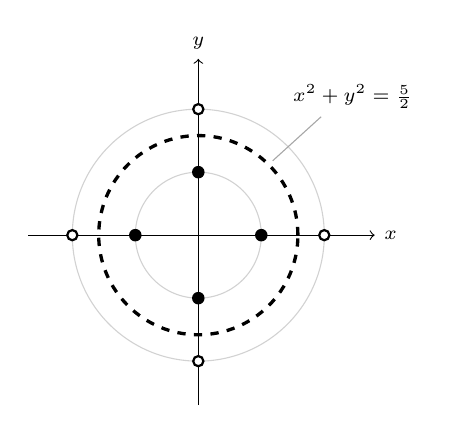
\begin{tikzpicture}[scale=0.8]
				% the two circles carrying the data
				\draw[gray!35] (0,0) circle (1);
				\draw[gray!35] (0,0) circle (2);
				% the separating circle
				\draw[dashed,very thick] (0,0) circle (1.5811);
				\node at (2.45,2.2) {\scriptsize $x^2+y^2=\frac{5}{2}$};
				\draw[gray!70] (1.95,1.88) -- (1.18,1.18);
				% axes
				\draw[->] (-2.7,0) -- (2.8,0) node[right] {\scriptsize $x$};
				\draw[->] (0,-2.7) -- (0,2.8) node[above] {\scriptsize $y$};
				% class +1
				\node[circle,fill=black,inner sep=1.6pt] at (1,0) {};
				\node[circle,fill=black,inner sep=1.6pt] at (-1,0) {};
				\node[circle,fill=black,inner sep=1.6pt] at (0,1) {};
				\node[circle,fill=black,inner sep=1.6pt] at (0,-1) {};
				% class -1
				\node[circle,draw,thick,fill=white,inner sep=1.3pt] at (2,0) {};
				\node[circle,draw,thick,fill=white,inner sep=1.3pt] at (-2,0) {};
				\node[circle,draw,thick,fill=white,inner sep=1.3pt] at (0,2) {};
				\node[circle,draw,thick,fill=white,inner sep=1.3pt] at (0,-2) {};
			\end{tikzpicture}
			\\[0.4em]
			{\scriptsize In the plane $(x,y)$: one class surrounds the other, and no line can separate them.}
		\end{minipage}
		\hfill
		\begin{minipage}[t]{0.46\textwidth}
			\centering
			\vspace{0pt}
			\begin{tikzpicture}[xscale=0.62,yscale=0.34]
				% the separating line
				\draw[dashed,very thick] (2.5,-5.3) -- (2.5,5.3);
				\node[above] at (2.5,5.3) {\scriptsize $u=\frac{5}{2}$};
				% axes
				\draw[->] (-0.8,0) -- (5.8,0) node[right] {\scriptsize $u$};
				\draw[->] (0,-5.7) -- (0,6.0) node[above] {\scriptsize $v$};
				\node[below] at (1,-5.4) {\scriptsize $u=1$};
				\node[below] at (4,-5.4) {\scriptsize $u=4$};
				% images of the class +1
				\node[circle,fill=black,inner sep=1.6pt] at (1,1) {};
				\node[circle,fill=black,inner sep=1.6pt] at (1,-1) {};
				\node[right,xshift=4pt] at (1,1) {\scriptsize $\times 2$};
				\node[right,xshift=4pt] at (1,-1) {\scriptsize $\times 2$};
				% images of the class -1
				\node[circle,draw,thick,fill=white,inner sep=1.3pt] at (4,4) {};
				\node[circle,draw,thick,fill=white,inner sep=1.3pt] at (4,-4) {};
				\node[right,xshift=4pt] at (4,4) {\scriptsize $\times 2$};
				\node[right,xshift=4pt] at (4,-4) {\scriptsize $\times 2$};
			\end{tikzpicture}
			\\[0.4em]
			{\scriptsize After $\phi$, in the plane $(u,v)$: a vertical line does the job. Each image carries two of the original points, marked $\times 2$.}
		\end{minipage}
	\end{center}
	The dashed circle on the left and the dashed line on the right are the same object, seen before and after the transformation.

	\section{Logistic Regression}

	The SVM outputs a hard decision: $+1$ or $-1$.
	Often we would rather have a \textbf{probability}: "this customer subscribes with probability $0.8$".
	This is what logistic regression provides.

	\paragraph{The model}
	\noindent\\
	We keep a linear function of the features, but we squash it into the interval $(0,1)$ with the \textbf{sigmoid} function
	$$
	\sigma(z) = \frac{1}{1 + e^{-z}}
	$$
	so that the model reads (here with labels written $0$ and $1$, which is the usual convention for this method)
	$$
	P(Y = 1 \mid X = x) = \sigma\left(\beta_0 + \beta_1 x\right) = \frac{1}{1 + e^{-(\beta_0 + \beta_1 x)}}
	$$
	The sigmoid is increasing, tends to $0$ at $-\infty$ and to $1$ at $+\infty$, and $\sigma(0) = \frac{1}{2}$.
	The decision boundary (where the model hesitates between the two classes) is therefore $\beta_0 + \beta_1 x = 0$.

	It also satisfies two identities that we will use constantly:
	$$
	\sigma(-z) = 1 - \sigma(z)
	\qquad \text{and} \qquad
	\sigma'(z) = \sigma(z)\left(1 - \sigma(z)\right)
	$$
	The first says $P(Y=0) = 1 - P(Y=1)$, as it must; the second is what makes the gradient below so simple.

	\paragraph{Why the sigmoid? Odds and log-odds}
	\noindent\\
	The sigmoid is not an arbitrary way of squashing a number into $(0,1)$.
	Recall that the \textbf{odds} of an event of probability $p$ are $\frac{p}{1-p}$ (a probability of $0.75$ gives odds of $3$, i.e. "3 to 1").
	If $p = \sigma(z)$, then, using $1 - p = \sigma(-z)$:
	$$
	\frac{p}{1-p} = e^{z}
	\qquad \text{that is} \qquad
	\log\left(\frac{p}{1-p}\right) = z = \beta_0 + \beta_1 x
	$$
	So logistic regression is a \textit{linear} model, not of the probability, but of the \textbf{log-odds}.
	This is what one should remember, for two reasons:
	\begin{itemize}
		\item it explains the shape of the model: a quantity that grows without bound (the log-odds) is converted into one that saturates (a probability);
		\item it is how the coefficients are read in practice.
		Adding one to $x$ adds $\beta_1$ to the log-odds, hence \textbf{multiplies the odds by $e^{\beta_1}$}, a factor that does not depend on where we started.
		A coefficient $\beta_1 = 0.64$ means "one extra unit multiplies the odds by $e^{0.64} \approx 1.9$", which is a sentence a client can act on, whereas "$\beta_1 = 0.64$" is not.
	\end{itemize}

	\paragraph{The cost function: log loss}
	\noindent\\
	To fit $\beta_0$ and $\beta_1$, we need to measure how wrong the model is.
	The usual choice is the \textbf{log loss} (also called cross-entropy):
	$$
	\mathcal{L}(\beta_0, \beta_1) = -\sum_{k=1}^{N} \Big[ y_k \log\left(p_k\right) + \left(1 - y_k\right) \log\left(1 - p_k\right) \Big]
	$$
	where $p_k = \sigma\left(\beta_0 + \beta_1 x_k\right)$.
	Since $y_k$ is $0$ or $1$, exactly one of the two terms survives for each point, and the contribution of the point is
	$$
	-\log\left(\text{probability the model assigned to the correct answer}\right)
	$$
	It is $0$ for a perfect prediction, and grows to $+\infty$ as the model becomes confidently wrong.
	This last property is what makes the log loss much more suitable than the squared error here: it punishes confident mistakes very severely.

	\paragraph{Minimizing the cost}
	\noindent\\
	Unlike the linear regression of Session 3, this minimization has no closed-form solution: we use \textbf{gradient descent}.
	The gradient takes a remarkably simple form:
	$$
	\frac{\partial \mathcal{L}}{\partial \beta_0} = \sum_{k=1}^{N} \left( p_k - y_k \right)
	\qquad \text{and} \qquad
	\frac{\partial \mathcal{L}}{\partial \beta_1} = \sum_{k=1}^{N} x_k \left( p_k - y_k \right)
	$$
	(the term $p_k - y_k$ is simply the error made on the $k$-th point), and the parameters are updated with
	$$
	\beta_0 \leftarrow \beta_0 - \eta \, \frac{\partial \mathcal{L}}{\partial \beta_0}
	\qquad \text{and} \qquad
	\beta_1 \leftarrow \beta_1 - \eta \, \frac{\partial \mathcal{L}}{\partial \beta_1}
	$$
	where $\eta$ is the learning rate.

	Note that at the minimum the gradient vanishes, which gives the two identities
	$$
	\sum_{k} p_k = \sum_{k} y_k
	\qquad \text{and} \qquad
	\sum_{k} x_k \, p_k = \sum_{k} x_k \, y_k
	$$
	They are a convenient way of checking a numerical result.

	\paragraph{Everything extends to more features}
	\noindent\\
	With $\vecx \in \R^n$ instead of a single number $x$, the model becomes
	$$
	P(Y = 1 \mid \vecx) = \sigma\left( \vecw \cdot \vecx + b \right)
	$$
	and all the formulas above hold, with $x_k$ replaced by $\vecxk$.
	The decision boundary $\vecw \cdot \vecx + b = 0$ is again a hyperplane: like the SVM, logistic regression is a \textit{linear} classifier (the two methods differ in what they optimize, not in the shape of their boundary).

	\paragraph{A worked example}
	\noindent\\
	We take the data of the exercise sheet: four students, the number of hours they studied, and whether they passed.

	\begin{center}
		\begin{tabular}{|c|c|}
			\hline
			Hours studied ($x$) & Pass ($y$) \\
			\hline
			$0$ & $0$ \\
			$4$ & $0$ \\
			$3$ & $1$ \\
			$8$ & $1$ \\
			\hline
		\end{tabular}
	\end{center}

	\noindent
	Writing the log loss for these four points, with $p_k = \sigma\left(\beta_0 + \beta_1 x_k\right)$, gives
	$$
	\mathcal{L}(\beta_0, \beta_1)
	= -\log\left(1 - p_1\right) - \log\left(1 - p_2\right) - \log\left(p_3\right) - \log\left(p_4\right)
	$$
	and, using $1 - \sigma(z) = \sigma(-z)$ and $-\log \sigma(z) = \log\left(1 + e^{-z}\right)$, everything can be written out explicitly:
	$$
	\begin{aligned}
		\mathcal{L}(\beta_0, \beta_1)
		= \ & \log\left(1 + e^{\beta_0}\right)
		+ \log\left(1 + e^{\beta_0 + 4\beta_1}\right) \\
		& + \log\left(1 + e^{-(\beta_0 + 3\beta_1)}\right)
		+ \log\left(1 + e^{-(\beta_0 + 8\beta_1)}\right)
	\end{aligned}
	$$
	The problem is to minimize this function of two variables over $\R^2$.
	It has no solution in closed form, so we hand it to a computer, which runs the gradient descent above (this is what the notebook does) and returns
	$$
	\beta_0 \approx -2.297,
	\qquad
	\beta_1 \approx 0.637,
	\qquad
	\mathcal{L} \approx 1.886
	$$

	\noindent
	The fitted model is then read as follows.
	\begin{itemize}
		\item The predicted probabilities of passing are $0.091$ for the student who studied $0$ hours, $0.404$ for $3$ hours, $0.562$ for $4$ hours and $0.942$ for $8$ hours.
		\item The decision boundary is at $x = -\frac{\beta_0}{\beta_1} \approx 3.6$ hours, which falls between the student who studied $3$ hours and passed and the one who studied $4$ hours and failed.
		\item Each extra hour of study multiplies the odds of passing by $e^{\beta_1} = e^{0.637} \approx 1.9$, which is the number quoted at the end of the paragraph on log-odds, and the form in which the result should be reported.
	\end{itemize}

	\noindent
	Note that the minimal cost is $1.886$ and not $0$: the student who studied $4$ hours failed while the one who studied $3$ hours passed, so no increasing function of $x$ can get all four right.
	The overlap of the two classes is a property of the data, not a failure of the method.

\end{document}
